 % The main file for CAMP reports
 % Don't put any content in here. 
 % Don't even include content files by using \input or \inlcude. 
 % Put your content to TEXT.TEX or include it there using \input.
 % Uses:
 %		SETTINGS.TEX	contains the settings for this document
 %		COMMANDS.TEX	contains commands which can be used while writing
 %		INFO.TEX			contains the author, title and so on for the cover
 %		COVER.TEX			formats the front cover of the document
 %		ABSTRACT.TEX	contains the abstract to be included (if needed)
 %		TEXT.TEX			contains the actual content of the document
 %		BIB.BIB				containt the BibTeX entries for the document
 
 
%% Draft document mode
%% Final document
\documentclass[11pt,a4paper,bibtotoc,idxtotoc,headsepline,footsepline,footexclude,BCOR12mm,DIV13]{scrbook}

%\documentclass[11pt,a4paper,bibtotoc,idxtotoc,headsepline,footsepline,footexclude,BCOR20mm,DIV10]{scrbook}

% KOMA-Optionen:
%  bibtotoc: include bibliography in table of contents
%  idxtotoc: include index in table of contents
%  headsepline: use horizontalline under heading
%  BCOR: binding correcion (Bindungskorrektur) (e.g.: BCOR5mm)
%  DIV: Number of sheet sections (used for layout) (e.g.: DIV12) 



% include title and author information for the cover
% Set here the title, authors and other stuff to be used for the cover
% This file is used by MAIN.TEX

% set title, authors and stuff for the cover
\def\doctype{Bachelorarbeit in Informatik}
\def\title{Implementation of an Android Framework for USB storage access without root rights}
\def\titleGer{Implementierung eines Android Frameworks f{\"u}r den Zugriff auf USB Speicher ohne Rootrechte}
\def\author{Magnus Jahnen}
\def\date{April 15, 2014}

% text to appear in the footer
\def\footertext{}

% include settings
% Included by MAIN.TEX
% Defines the settings for the CAMP report document

\renewcommand{\sectfont}{\normalfont \bfseries}        % Schriftart der Kopfzeile

% manipulate footer
\usepackage{scrpage2}
\pagestyle{scrheadings}
\ifoot[\footertext]{\footertext} % \footertext set in INFO.TEX
%\setkomafont{pagehead}{\normalfont\rmfamily}
\setkomafont{pagenumber}{\normalfont\rmfamily}

\usepackage{url}

%% allow sophisticated control structures
\usepackage{ifthen}

% use Palatino as default font
\usepackage{palatino}

% enable special PostScript fonts
\usepackage{pifont}

% make thumbnails
\usepackage{thumbpdf}

%to use the subfigures
\usepackage{subfigure}


\usepackage{colortbl}


%% show program code\ldots
%\usepackage{verbatim}
%\usepackage{program}

%% enable TUM symbols on title page
\usepackage{styles/tumlogo}


\usepackage{multirow}

%% use colors
\usepackage{color}

%% make fancy math
\usepackage{amsmath}
\usepackage{amsfonts}
\usepackage{amssymb}
\usepackage{textcomp}
\usepackage{yhmath} % f�r die adots 
%% mark text as preliminary
%\usepackage[draft,german,scrtime]{prelim2e}

%% create an index
\usepackage{makeidx}

% for the program environment
\usepackage{float}

%% load german babel package for german abstract
%\usepackage[german,american]{babel}
\usepackage[german,english]{babel}
\selectlanguage{english}

% use german characters as well
\usepackage[latin1]{inputenc}       % allow Latin1 characters

% use initals dropped caps - doesn't work with PDF
%\usepackage{dropping}


\usepackage{styles/shortoverview}
%----------------------------------------------------
%      Graphics and Hyperlinks
%----------------------------------------------------

%% check for pdfTeX
\ifx\pdftexversion\undefined
 %% use PostScript graphics
 \usepackage[dvips]{graphicx}
 \DeclareGraphicsExtensions{.eps,.epsi}
 \graphicspath{{figures/}{figures/review}} 
 %% allow rotations
 \usepackage{rotating}
 %% mark pages as draft copies
 %\usepackage[english,all,light]{draftcopy}
 %% use hypertex version of hyperref
 \usepackage[hypertex,hyperindex=false,colorlinks=false]{hyperref}
\else %% reduce output size \pdfcompresslevel=9
 %% declare pdfinfo
 %\pdfinfo { 
 %  /Title (my title) 
 %  /Creator (pdfLaTeX) 
 %  /Author (my name) 
 %  /Subject (my subject	) 
 %  /Keywords (my keywords)
 %}
 %% use pdf or jpg graphics
 \usepackage[pdftex]{graphicx}
 \DeclareGraphicsExtensions{.jpg,.JPG,.png,.pdf,.eps}
 \graphicspath{{figures/}} 
 
 %% Load float package, for enabling floating extensions
 \usepackage{float}
 
 %% allow rotations
 \usepackage{rotating}
 %% use pdftex version of hyperref
 \usepackage[pdftex,colorlinks=true,linkcolor=red,citecolor=red,%
 anchorcolor=red,urlcolor=red,bookmarks=true,%
 bookmarksopen=true,bookmarksopenlevel=0,plainpages=false%
 bookmarksnumbered=true,hyperindex=false,pdfstartview=%
 ]{hyperref}
%
%\usepackage[pdftex,colorlinks=false,linkcolor=red,citecolor=red,%
% anchorcolor=red,urlcolor=red,bookmarks=true,%
% bookmarksopen=true,bookmarksopenlevel=0,plainpages=false%
% bookmarksnumbered=true,hyperindex=false,pdfstartview=%
% ]{hyperref}
\fi




%% Fancy chapters
%\usepackage[Lenny]{fncychap}
%\usepackage[Glenn]{fncychap}
%\usepackage[Bjarne]{fncychap}

%\usepackage[avantgarde]{quotchap}

% set the bibliography style
%\bibliographystyle{styles/bauermaNum}
%\bibliographystyle{alpha}
\bibliographystyle{plain}

% include commands
% Commands to be used within the TUM report document
% Included by MAIN.TEX
% Please include your own cool commands here. 
% Be only sure to comment it sufficiently so others can use it.

%-------------------------------------------------------------
%                      Own Commands
%-------------------------------------------------------------


%-------------------------------------------------------------
% math stuff -------------------------------------------------

% nice R, N, C
\newcommand{\nat}{\mathbb{N}}
\newcommand{\real}{\mathbb{R}}
\newcommand{\compl}{\mathbb{C}}



% norm
\newcommand{\norm}[1]{\left\| #1 \right\|}

% un demi
\newcommand{\half}{\frac{1}{2}}

% parantheses
\newcommand{\parenth}[1]{ \left( #1 \right) }
\newcommand{\bracket}[1]{ \left[ #1 \right] }
\newcommand{\accolade}[1]{ \left\{ #1 \right\} }
%\newcommand{\angle}[1]{ \left\langle  #1 \right\rangle }

% partial derivative: %#1 function, #2 which variable
% simple / single line version
\newcommand{\pardevS}[2]{ \delta_{#1} f(#2) }
% fraction version
\newcommand{\pardevF}[2]{ \frac{\partial #1}{\partial #2} }

% render vectors: 3 and 4 dimensional
\newcommand{\veciii}[3]{\left[ \begin{array}[h]{c} #1 \\ #2 \\ #3	\end{array} \right]}
\newcommand{\veciv}[4]{\left[ \begin{array}[h]{c} #1 \\ #2 \\ #3 \\ #4	\end{array} \right]}

% render matrices: 3  dimensional (arguments in row first order)
\newcommand{\matiii}[9]{\left[ \begin{array}[h]{ccc} #1 & #2 & #3 \\ #4 & #5 & #6 \\ #7 & #8 & #9	\end{array} \right]}
%DOESN'T WORK,DON'T KNOW WHY \newcommand{\mativ}[16]{\left[ \begin{array}[h]{cccc} #1 & #2 & #3 & #4 \\ #5 & #6 & #7 & #8 \\ #9 & #10 & #11 & #12 \\ #13 & #14 & #15 & #16 \end{array} \right]}


%-------------------------------------------------------------
%-------------------------------------------------------------


%-------------------------------------------------------------
% some abreviations ------------------------------------------
\newcommand{\Reg}{$^{\textregistered}$}
\newcommand{\reg}{$^{\textregistered}$ }
\newcommand{\Tm}{\texttrademark}
\newcommand{\tm}{\texttrademark~}
\newcommand {\bsl} {$\backslash$}

%-------------------------------------------------------------
%-------------------------------------------------------------


%-------------------------------------------------------------
% formating --------------------------------------------------

% Theorem & Co environments and counters
\newtheorem{theorem}{Theorem}[chapter]
\newtheorem{lemma}[theorem]{Lemma}
\newtheorem{corollary}[theorem]{Corollary}
\newtheorem{remark}[theorem]{Remark}
\newtheorem{definition}[theorem]{Definition}
\newtheorem{equat}[theorem]{Equation}
\newtheorem{example}[theorem]{Example}
\newtheorem{algorithm}[theorem]{Algorithm}

% inserting figures
\newcommand{\insertfigure}[4]{ % Filename, Caption, Label, Width percent of textwidth
	\begin{figure}[htbp]
		\begin{center}
			\includegraphics[width=#4\textwidth]{#1}
		\end{center}
		\vspace{-0.4cm}
		\caption{#2}
		\label{#3}
	\end{figure}
}




% referecing figures

\newcommand{\refFigure}[1]{ %label
	figure \ref{#1}
}
\newcommand{\refChapter}[1]{ %label
	chapter \ref{#1}
}

\newcommand{\refSection}[1]{ %label
	section \ref{#1}
}

\newcommand{\refParagraph}[1]{ %label
	paragraph \ref{#1}
}

\newcommand{\refEquation}[1]{ %label
	equation \ref{#1}
}

\newcommand{\refTable}[1]{ %label
	table \ref{#1}
}




\newcommand{\rigidTransform}[2]
{
	${}^{#2}\!\mathbf{H}_{#1}$
}

%code, in typewriter
\newcommand{\code}[1]
 {\texttt{#1}}

% comment that appears on the border - very practical !!!
\newcommand{\comment}[1]{\marginpar{\raggedright \noindent \footnotesize {\sl #1} }}

% page clearing
\newcommand{\clearemptydoublepage}{%
  \ifthenelse{\boolean{@twoside}}{\newpage{\pagestyle{empty}\cleardoublepage}}%
  {\clearpage}}


%-------------------------------------------------------------
%-------------------------------------------------------------


\newcommand{\etAl}{\emph{et al.}\mbox{ }}


%\makeindex
	%% inter line spacing
%\linespread{1.0}

\makeglossary

\begin{document}

	\frontmatter
	
	
	% The front cover for the TUM report document.
% Included by MAIN.TEX


%--------------------------------------------------
% The Front Cover
%--------------------------------------------------

% The front cover for the TUM document.
% Included by MAIN.TEX


%--------------------------------------------------
% The Front Cover
%--------------------------------------------------

% correct BCOR - undo at the end !!!
\def\bcorcor{0.15cm}
\addtolength{\hoffset}{\bcorcor}

\thispagestyle{empty}

 \vspace{4cm}
\begin{center}
	       \oTUM{4cm}
	   
	   \vspace{5mm}     
	   \huge FAKULT{\"A}T F{\"U}R INFORMATIK\\ 
	   \vspace{0.5cm}
	 \large DER TECHNISCHEN UNIVERSIT{\"A}T M{\"U}NCHEN\\
    \vspace{1mm}
        
	\end{center}
		

\vspace{15mm}
\begin{center}

   {\Large \doctype}

  \vspace{20mm}
  
  {\huge\bf \title}\\%[3ex]
  
  
  \vspace{15mm}
  
  
  {\LARGE  \author}
  
  \vspace{10mm}
  
  \begin{figure}[h!]
  \centering
   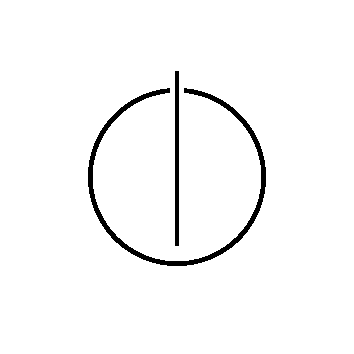
\includegraphics[width=4cm]{styles/informat.png}
  \end{figure}
  
  \end{center}
%	\clearemptydoublepage
%	
%	% The titlepage for the CAMP report document.
% Included by MAIN.TEX


%--------------------------------------------------
% The title page
%--------------------------------------------------

% correct BCOR - undo at the end !!!
\def\bcorcor{0.15cm}
\addtolength{\hoffset}{\bcorcor}

\thispagestyle{empty}

 \vspace{10mm}
\begin{center}
	       \oTUM{4cm}
	   
	   \vspace{5mm}     
	   \huge FAKULT{\"A}T F{\"U}R INFORMATIK\\ 
	   \vspace{0.5cm}
	 \large DER TECHNISCHEN UNIVERSIT{\"A}T M{\"U}NCHEN\\
        
	\end{center}
		

\vspace{10mm}
\begin{center}

   {\Large \doctype}

  \vspace{10mm}
  
  {\LARGE \title}\\
  
  
  \vspace{10mm}
  
  
  {\LARGE  \titleGer}\\
  
  
  \vspace{10mm}

    %\hfill
    \begin{tabular}{ll}
	   \Large Author:     & \Large \author \\[2mm]
	   \Large Supervisor:    & \Large Prof. Dr. Uwe Baumgarten \\[2mm]				
	   \Large Advisor:	& \Large Nils Kannengie{\ss}er, M.Sc. \\[2mm]
	   \Large Date:       & \Large April 15, 2014
	 \end{tabular}
	 
	 \vspace{5mm}
	 
	 \begin{figure}[h!]
  \centering
   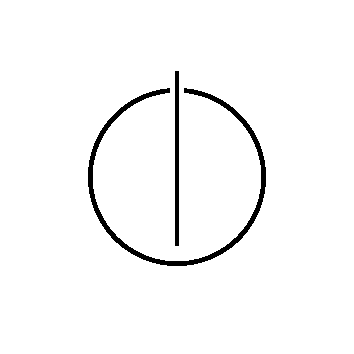
\includegraphics[width=4cm]{styles/informat.png}
  \end{figure}
   

\end{center}

% undo BCOR correction
\addtolength{\hoffset}{\bcorcor}
	
	
%	\input{components/cover_maschmeyer}
	\clearemptydoublepage
	
	% The titlepage for the CAMP report document.
% Included by MAIN.TEX


%--------------------------------------------------
% The title page
%--------------------------------------------------

% correct BCOR - undo at the end !!!
\def\bcorcor{0.15cm}
\addtolength{\hoffset}{\bcorcor}

\thispagestyle{empty}

 \vspace{10mm}
\begin{center}
	       \oTUM{4cm}
	   
	   \vspace{5mm}     
	   \huge FAKULT{\"A}T F{\"U}R INFORMATIK\\ 
	   \vspace{0.5cm}
	 \large DER TECHNISCHEN UNIVERSIT{\"A}T M{\"U}NCHEN\\
        
	\end{center}
		

\vspace{10mm}
\begin{center}

   {\Large \doctype}

  \vspace{10mm}
  
  {\LARGE \title}\\
  
  
  \vspace{10mm}
  
  
  {\LARGE  \titleGer}\\
  
  
  \vspace{10mm}

    %\hfill
    \begin{tabular}{ll}
	   \Large Author:     & \Large \author \\[2mm]
	   \Large Supervisor:    & \Large Prof. Dr. Uwe Baumgarten \\[2mm]				
	   \Large Advisor:	& \Large Nils Kannengie{\ss}er, M.Sc. \\[2mm]
	   \Large Date:       & \Large April 15, 2014
	 \end{tabular}
	 
	 \vspace{5mm}
	 
	 \begin{figure}[h!]
  \centering
   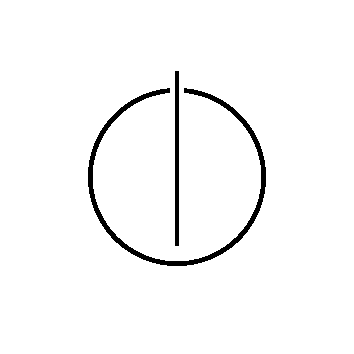
\includegraphics[width=4cm]{styles/informat.png}
  \end{figure}
   

\end{center}

% undo BCOR correction
\addtolength{\hoffset}{\bcorcor}
	
	
	\clearemptydoublepage


\thispagestyle{empty}
\selectlanguage{german}
	\vspace*{0.8\textheight}
	\noindent
	Ich versichere, dass ich diese Bachelorarbeit selbst{\"a}ndig verfasst und nur 
	die angegebenen \\Quellen und Hilfsmittel verwendet habe.
	
	\vspace{15mm}
	\noindent
	M{\"u}nchen, den \today \hspace{5cm} \author
\selectlanguage{english}
\newpage
	
	\clearemptydoublepage
\phantomsection
\addcontentsline{toc}{chapter}{Acknowledgements}	


%\chapter*{Acknowledgements}

\vspace*{2cm}

\begin{center}
{\Large \bf Acknowledgments}
\end{center}

\vspace{1cm}




If someone contributed to the thesis... might be good to thank them here.
	
	% Abstract for the TUM report document
% Included by MAIN.TEX


\clearemptydoublepage
\phantomsection
\addcontentsline{toc}{chapter}{Abstract}	





\vspace*{2cm}
\begin{center}
{\Large \bf Abstract}
\end{center}
\vspace{1cm}

An abstracts abstracts the thesis!

	\tableofcontents
  
  \clearemptydoublepage

\phantomsection
\addcontentsline{toc}{chapter}{Outline of the Thesis}

\begin{center}
	\huge{Outline of the Thesis}
\end{center}




%--------------------------------------------------------------------
\section*{Part I: Introduction and Theory}

\noindent {\scshape Chapter 1: Introduction}  \vspace{1mm}

\noindent  This chapter presents an overview of the thesis and its purpose. \\

\noindent {\scshape Chapter 2: Basics about USB}  \vspace{1mm}

\noindent  This chapter describes the basics about USB, how it is structured and how does it generally work.   \\

\noindent {\scshape Chapter 3: USB on Android}  \vspace{1mm}

\noindent  Chapter 3 introduces the reader to the USB API on Android. How can USB devices be enumerated and accessed, and how can the communication be initiated? \\

\noindent {\scshape Chapter 4: USB Mass storage class}  \vspace{1mm}

\noindent  This chapter gives an overview of the USB Mass storage class. The main goal is to understand SCSI commands to communicate with the device and read and write from and to its storage. \\

\noindent {\scshape Chapter 5: File systems}  \vspace{1mm}

\noindent  Chapter 5 discusses the approach of file system in general, and then gives a detailed description of how FAT32 from Microsoft works. \\

%--------------------------------------------------------------------
\section*{Part II: Implementation}

\noindent {\scshape Chapter 6: Purpose and Overview}  \vspace{1mm}

\noindent  This chapter presents the purpose and requirements for the implementation. It also provides a short overview of the implementation. \\

\noindent {\scshape Chapter 7: Inside the packages}  \vspace{1mm}

\noindent  Chapter 7 gives a deeper insight into the developed framework and its packages, classes and interaction between the important parts. \\

\noindent {\scshape Chapter 8: Current status}  \vspace{1mm}

\noindent  Short summary of the current status of the framework, especially what things are supported and which are not. \\

\section*{Part III: Quality Management}

\noindent {\scshape Chapter 9: Testing}  \vspace{1mm}

\noindent  This chapter presents the results of different tests on various devices. \\


	\mainmatter
	
	
		% ---------------------------------------------------------------------------
		%
		%Introduction and Background Theory
		%
		% ---------------------------------------------------------------------------
		\part[Introduction and Theory]{Introduction and Theory}
		\label{part:introAndBackgroundTheory}
		\chapter{Introduction}
\label{chapter:Introduction}



Since Android 3.1 a lot of Android devices come with USB host support (USB on the go). That means a normal Android tablet or phone can not only act as a USB client when connected to a computer. It can also act as a USB host for periphals by powering the bus with the needed 5 Volt and changing into a USB host mode and enumerating connected USB devices\cite{android_usb_host}. Android currently supports interrupt, bulk and control transfers (isochronous transfers are currently unsupported). That means nearly every USB device can, theoretically, be used with an Android device (Webcams or Audio devices mostly use isochronous transfers and can thus not be used at the moment). The Android host API easily allows to communicate with connected USB devices, meaning you can write your own high level USB driver in Java.\\
Thus the idea of connecting a USB mass storage device like USB sticks or external HDDs is not that far away. Especially when you look at recent occurences where a lot of devices miss a slot for external SD-Cards and only offer a solid internal storage. Unfortunately the stock Android comes without support for USB storage devices. That means when you are connecting your mass storage device nothing will happen. You can not access the data via a file manager or something similiar. On rooted devices this is possible because the alternative Android ROMs provide support for it. But with the Android USB Host API it should also be possible to access such devices with out rooting the device and flashing an alternative ROM. The only thing you have to do is to implement the low level USB communication via eg. bulk transfers and the abtraction of directorys and files via a filesystem. This can of course also be done in Java and not only in plain C.\\
Currently there are two applications in the Google Play Store which allow accessing mass storage devices without root rights! First there is a plugin for the Total Commander called USB-Stick Plugin-TC. The plugin extends the Total Commander application by USB mass storage access. It currently supports FAT12, FAT16, FAT32 exFAT and NTFS (read only). There is a free trial version available. The second application is called Nexus Media Importer. It supports FAT16, FAT32 and NTFS (also read only). There is no free trial verson available. In general both apps support USB sticks, external HDDs and card readers.\\
The problem both applications have is that there is no solution to access the mass storage from other apps. That means all accessed data has to be cached and copied to the internal storage before any other app can access it. These limitations are annoying but it seems that they are impossible to overcome.\\
Both applications are proprietary and thus do not offer the ability to look into and change the source code. Therefore an open source Android Framework for accessing mass storage devices is developed in this bachelor thesis. The license is the very liberale Apache License, Version 2.0, Android is also licensed under.\\
Due to the same license it would be possible that Google integrates this solution into the official Android. Indeed there are some disadvantages which makes the integration unlikely. First all needed things, like filesystems (eg. FAT32) or the SCSI transparent command set, for mounting USB mass storage are already implemented in the underlying Linux kernel. Google just deactivated the support for it. Next with our solution only apps which use our framework can access USB storage devices. It would be much nicer if the conncected devices would be mounted in the normal unix filesystem like sd cards. For example under /mnt/usbstick0. This would make it possible for other apps easily access data from USB mass storage without extra changes to the application. Due to this I think that is very unlikely that Google will integrate this framework into the official Android!
 
\section{Basics about USB}

USB means universal serial bus interface is a serial bussystem to connect a computer with external devices. The first version was introduced by Intel and now the specification is done by the USB Implementers Forum (USB-IF). The USB-IF is a corporation founded by various companies which work non-profit on the USB specification. In USB there exists one USB host controller (eg. computer) which initiates the connection and comunication and multiple clients (slaves). The client only sends data when the host aks for it. The USB host ist responsible for powering the connected client, thus an external power source is only in some special cases necessary.

\subsection{Client device hierarchy}

A USB client can be structured in four different USB descriptors. The device, configuration, interface and endpoints.\\
The device descriptor represents the USB device as a hole device which is connected to the USB bus. This can be for example a loud speaker with volume control buttons.\\
The configuration descriptor represents the current state of the USB device. This can for example be standby or active.\\
A USB Interface descriptor describes every logical device which belongs to the USB device. Often USB devices consist of multiple logical device units. For example a loud speaker is the first logical device and the control buttons to adjust the volume are the second logical device.\\
Lastly there are the endpoint descriptors which represent unidirectional communication pipes. This is where the actual communication happens. The other descriptors are only to describe the USB device. Endpoints can be of type IN (device to host) or OUT (host to device). Additional tehre are four different types of endpoints to fit different requirements when communicating.\\

\subsection{Endpoints}

Every USB device has different requirements towards the underlying communication pipe. To satisfy the different needs the USB protocol offers four different types of communicaton (endpoints).\\
Control endpoints are used to configure the device and retrieve status information. These transfers are typically very small. Every device has a control endpoint called endpoint 0 which plays an important role at insertion time.\\
Interrupt transfers carry a small amount of data to the host everytime the host aks for it. This happens at a fixed rate resulting in a fixed and guarenteed bandwidth. These transfers are used by Human interface devices (eg. mouse, keyboard, gamepads) which need a low latency and a low paket size.\\
Next there are bulk endpoints. These are useful when the amount of data transferred varies often and happens infrequently. The remaining bandwidth the bus provides is used. Hence there is no guarantee on bandwith or latency. However bulk transfers offer consistent data transfers, meaning that no data is lost. Typically used for printers, network or mass storage devices. Everywhere where data loss is unacceptable and no guarenteed bandwith is needed.\\
Finally there are the isochronous transfers. They offer a guarenteed bandwith while resigning consistency. The guarenteed bandwith is mostly as fast as possible and valueable for real time transfers (eg. audio or video). Mostly these transfers are used for Webcams or Audio devices (eg. external audio cards/audio interfaces).\\

\subsection{USB on the go}

As already mentioned in the USB communication there is always a host (master) and a client (device). The host initates the communication and acts as a master. That means the client is not allowed to send data at every time, it can only send data when the host explicitly asks to do so! The client is only able to signal that it requires attention. Then the host must react and ask for receiving data. When connecting a smartphone or tablet to the computer the computer acts as the host and the smartphone as the client device. That means the smartphone normally acts as a client device and not as the USB host. In our constellation, however, it has obvisously to act as a host. \\
For that reason the USB-IF developed the USB on the go (USB OTG) featur in 2001. It is part of the USB 2.0 specification. This feature allows a USB device to act as a client or either a host depending on the present situation. To use the USB OTG mode a special USB OTG adapter is needed. This is necessary for two reasons. Apriori for signalling that the smartphone should now act as a host and not as usual as a client and secondly because most smartphones and tables do not provide a normal USB port of type A. Instead they offer a mini (older devices) or micro port of type A and B. 

\section{USB Mass storage class}

Most USB devices are very similiar. To reduce development effort and allow OS designers offering generic drivers for a great range of different devices a lot of device types are standardized. These different types are called classes in USB. There are for example standardizations for printers, USB hubs, Audio or Video Devices, Human Interface devices and mass storage devices. We will now concentrate on the mass storage class.\\
Every mass storage device has at least one interface descriptor with the class code 08h, which stands for the mass storage class. Note that the mass storage class is not defined in the device descriptor! The USB interface has exactly two endpoint descriptors. One IN endpoint to read from the device and one OUT endpoint to write to the device. Reading and writing in this case does not neccessarily mean reading or writing on the actual storage medium, but we will see that later on.\\
There are several sources regarding the mass storage class. It exists the bulk-only transport mechanism which is the most popular one. All newer devices follow these standard. The there is the Control/Bulk/Interrupt (CBI) standard and the UFI Command specification, which are no longer important. In the end the are some mechanisms to allow booting from removable media. We will concentrate on the bulk-only transport short BBB.

\subsection{Bulk-only Transport}

Unlike the name suggests there are two control requests in the BBB specification. The first one is a reset request to make the device becomming ready for the next command. The second is used to get the maximun LUN (Get Max LUN request). This requests tells about the number of standalone logical units the mass storage device supports.\\
Like saif before the interface class has to be set to 08h for the mass storage class. The subclass of the interface descriptor can have different values and specifies the supported protocols used to read and write data to the mass storage. Table \ref{table:subclass} gives an overview of the different protocol.

\begin{table}[ht]
\caption{Overview subclass protocols}
\centering
\begin{tabular}{|l|l|}
\hline\hline
01h & Reduced Block Coammnds (RBC) \\ \hline
02h & SFF-8020i, MMC-2 (ATAPI) (CD/DVD drives) \\ \hline
03h & QIC-157 (tape drives) \\ \hline
04h & USB Floppy Interface (UFI) \\ \hline
05h & FF-8070i (ATAPI removable rewritable media devices) \\ \hline
06h & SCSI transparent command set \\ \hline
\end{tabular}
\label{table:subclass}
\end{table}

For our purpose the SCSI transparent command set is the most important one. The RBC is even not implemented in Windows, but in the Linux kernel. The other protocols refer to other types of storage media we do not want to cover.
		
		
		%
		%% ---------------------------------------------------------------------------
		%%
		%% Fully Automated Calibration for Ultrasound
		%%
		%%% ---------------------------------------------------------------------------
		\part[The 2nd Part]{The Second Part}
		\label{part:secondP}
		
		
		% ---------------------------------------------------------------------------
		%
		% Appendix
		%
		% ---------------------------------------------------------------------------
		
		\part*{Appendix}
		\addcontentsline{toc}{part}{Appendix}
		
		\appendix %---------------------------------------
		
		\chapter{Detailed Descriptions}
%\section{Detailed Validation Results}
\label{chapter:DetailedDescriptions}
Here come the details that are not supposed to be in the regular text.
		
	


  \clearemptydoublepage
  
	\bibliography{bibliography/literature}
	
 
\end{document}

